\subsubsection{Les Contrôleurs}
\label{subsubsec:controleur}

Afin de garantir le bon fonctionnement de notre application, nous avons implémenté un contrôleur qui permet de gérer les interactions entre les différentes parties de notre application. Le contrôleur est composé de plusieurs classes qui permettent de gérer les différents menus, les paramètres audio, les règles du jeu, la création de partie, la partie en elle-même, etc. C'est ce qui lie notre MVC et permet de faire fonctionner notre application.

\paragraph{Les mouvements}

Nous avons décidé de créer une interface \textbf{\textit{MazeController}} qui est implémentée par \textbf{\textit{MazeControllerImplementation}}. Cette interface
contient toutes les méthodes qui permettent de gérer les mouvements du joueur.


Pour déplacer les joueurs nous utilisons principalement la voix, mais nous donnons aussi au jouer le choix d'utiliser le clavier. Pour gérer ces deux types de mouvements
nous utilisons deux classes:
\begin{itemize}
    \item \textbf{\textit{VoiceMovementController}} qui permet de gérer les mouvements du joueur avec la voix
    \item \textbf{\textit{KeyboardMovementController}} qui permet de gérer les mouvements du joueur avec le clavier
\end{itemize}
Ces deux classes sont utilisées en composition dans la classe \textbf{\textit{MazeControllerImplementation}} qui permet de gérer les mouvements du joueur.


\paragraph{Les menus}

Afin de gérer la fenêtre de notre jeu et de naviguer entre les différents menus, nous avons créé la classe \textbf{\textit{MenuFrameHandler}}. Cette classe se charge de changer le \textbf{\textit{JPanel}} de la fenêtre principale de notre application, qui est une \textbf{\textit{JFrame}}.


\paragraph{L'écran d'accueil} (\ref{fig:StartMenu})

Nous avons un écran d'accueil, géré par la classe \textbf{\textit{StartMenu}}, qui possède des boutons pour:

\begin{itemize}
    \item Aller au menu de création de partie
          \vcenteredinclude[height=5mm]{ressources/Implementation/Labyrinthe/Controleur/StartButton.png}
    \item Aller au menu des paramètres audio
          \vcenteredinclude[height=5mm]{ressources/Implementation/Labyrinthe/Controleur/Settings.png}
    \item Afficher les règles du jeu
          \vcenteredinclude[height=5mm]{ressources/Implementation/Labyrinthe/Controleur/QuestionMark.png}
          %   \item Afficher les crédits
          % \item Quitter le jeu
\end{itemize}

Les différents éléments graphiques tels que le GIF et les images des boutons sont gérés par la classe \textbf{\textit{JPanelWithImages}}.

\begin{figure}[h!]
    \centering
    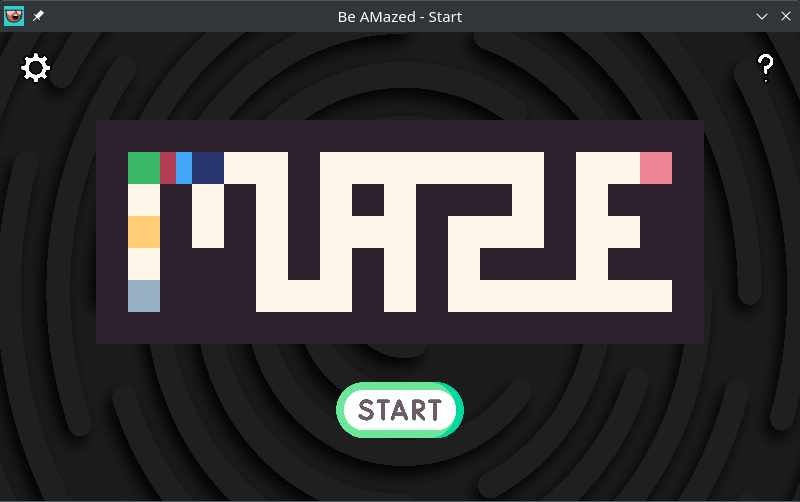
\includegraphics[width=10cm]{ressources/Implementation/Labyrinthe/Controleur/StartMenu.png}%
    \caption{L'écran d'accueil}
    \label{fig:StartMenu}
\end{figure}
\FloatBarrier

\paragraph{Les paramètres audio} (\ref{fig:Rules})

La vue des paramètres audio sera abordée dans la section \ref{subsec:son}.

\paragraph{Les règles de jeu}

Les règles du jeu sont affichées en anglais dans une fenêtre qui se superpose à celle du menu principal.

\begin{figure}[h!]
    \centering
    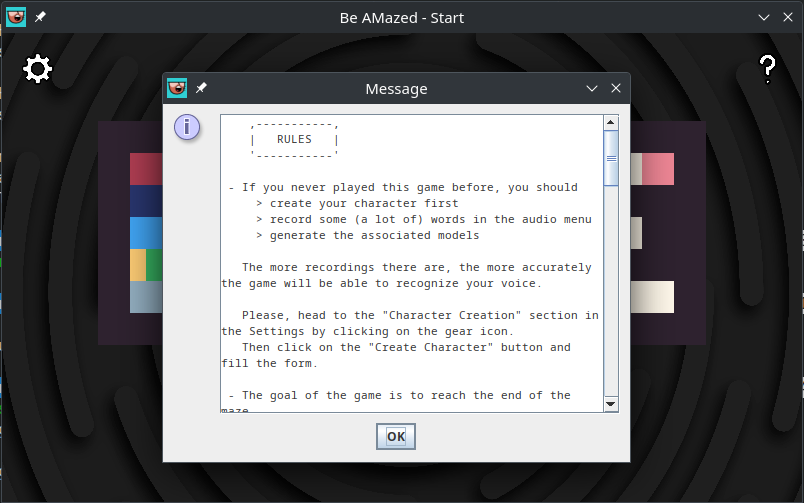
\includegraphics[width=10cm]{ressources/Implementation/Labyrinthe/Controleur/Rules.png}%
    \caption{Les règles du jeu}
    \label{fig:Rules}
\end{figure}
\FloatBarrier

\paragraph{La création de partie}

La création de la partie se décompose en plusieurs étapes et dispose de plusieurs éléments graphiques afin de permettre à l'utilisateur de choisir les paramètres de la partie qu'il souhaite jouer (nombre de joueurs, difficulté, etc.) le plus facilement possible. Cela est rendu possible par la classe \textbf{\textit{SettingsMenu}} qui gère l'ensemble des menus de paramétrage de la partie.

\subparagraph*{Le choix du mode de jeu} (\ref{fig:ModeSelection})

Le menu déroulant permet de choisir entre les différents modes de jeu disponibles. Il est géré par la classe \textbf{\textit{SelectionPanel}}.

\begin{figure}[h!]
    \centering
    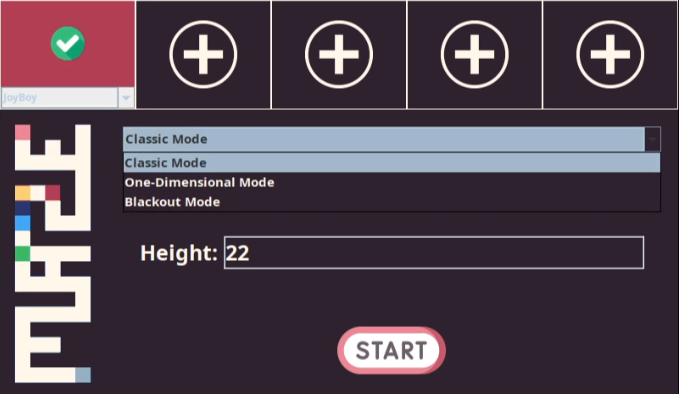
\includegraphics[width=10cm]{ressources/Implementation/Labyrinthe/Controleur/SettingsMenu_ModeList.png}%
    \caption{Menu déroulant des modes de jeu}
    \label{fig:ModeSelection}
\end{figure}
\FloatBarrier

Pour les afficher les menus des différents modes de jeu, nous avons des classes qui permettent de gérer les différents panels concernés. Ces classes sont des implémentations de l'interface  \textbf{\textit{PanelHandler}} et sont créées grâce à la classe  \textbf{\textit{PanelHandlerFactory}}.

\subparagraph*{Le mode Classique} (\ref{fig:ClassicMode})

Grâce à la classe \textbf{\textit{ClassicPanelHandler}}, nous avons à disposition deux entrées texte permettant de choisir la taille du labyrinthe.

\begin{figure}[h!]
    \centering
    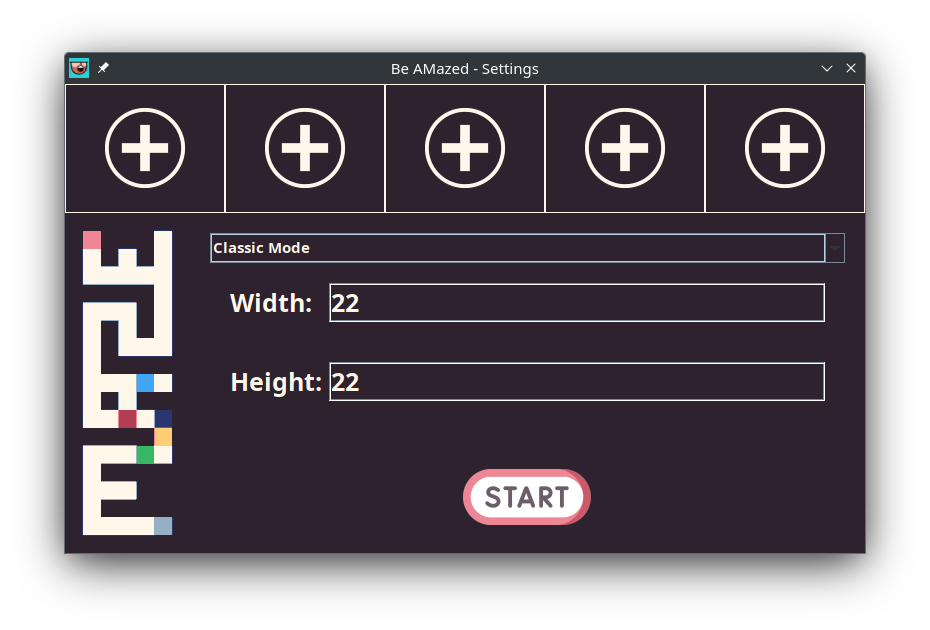
\includegraphics[width=10cm]{ressources/Implementation/Labyrinthe/Controleur/SettingsMenu_ClassicMode.png}
    \caption{Paramètres du mode classique}
    \label{fig:ClassicMode}
\end{figure}
\FloatBarrier

\subparagraph*{Le mode Blackout} (\ref{fig:BlackoutModeDifficulty})

Grâce à la classe \textbf{\textit{BlackoutPanelHandler}}, le mode Blackout possède 3 difficultés : \textbf{\textit{EASY}}, \textbf{\textit{MEDIUM}} et \textbf{\textit{HARD}} qu'on peut sélectionner grâce à un menu déroulant.

\begin{figure}[h!]
    \centering
    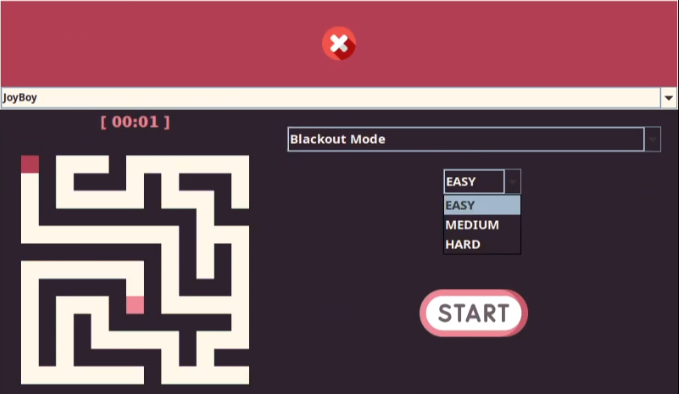
\includegraphics[width=10cm]{ressources/Implementation/Labyrinthe/Controleur/SettingsMenu_BlackoutMode_Difficulty.png}
    \caption{Paramètres du mode Blackout}
    \label{fig:BlackoutModeDifficulty}
\end{figure}
\FloatBarrier

\newpage

\subparagraph*{La préparation des joueurs} (\ref{fig:PlayerSelection})

Grâce aux classes \textbf{\textit{PlayerPanel}}, \textbf{\textit{PlayerSelectionPanel}} et \textbf{\textit{UserSelector}}, nous pouvons choisir le nombre de joueurs, leur couleur et leur nom parmi la liste des joueurs qui ont déjà été crées précédemment.

Tout d'abord, pour ajouter un joueur, on clique sur une case "+". Une case de couleur s'affichera. Ensuite on choisit le nom du joueur dans la liste déroulante. Enfin il faut confirmer que le joueur est prêt en cliquant sur sa case.

\begin{figure}[h!]
    \centering
    \begin{subfigure}{6.5cm}
        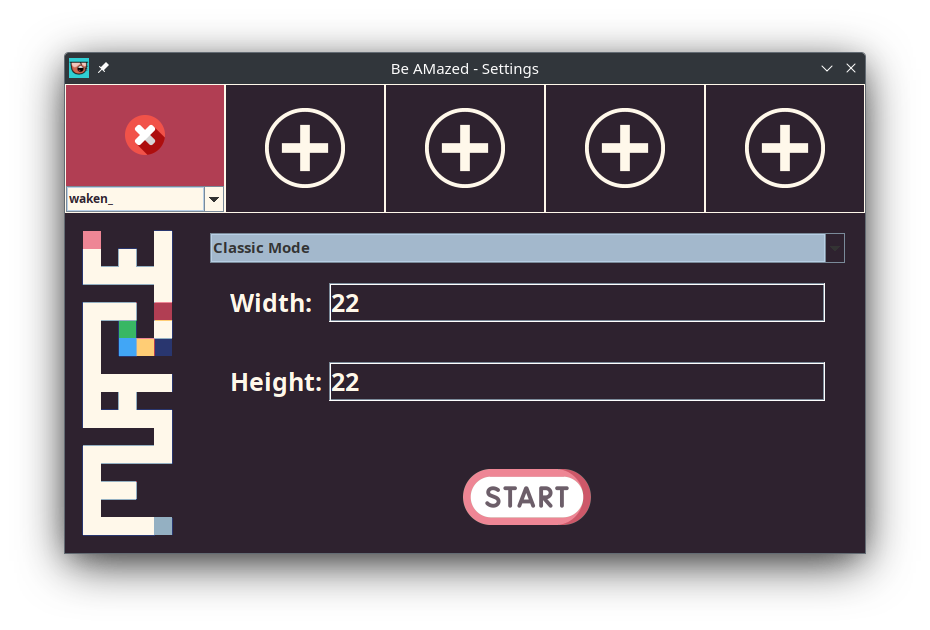
\includegraphics[width=6.5cm]{ressources/Implementation/Labyrinthe/Controleur/SettingsMenu_NotReady.png}%
        \caption{Joueur pas prêt}
        \label{fig:PlayerNotReady}
    \end{subfigure}
    \qquad
    \begin{subfigure}{6.5cm}
        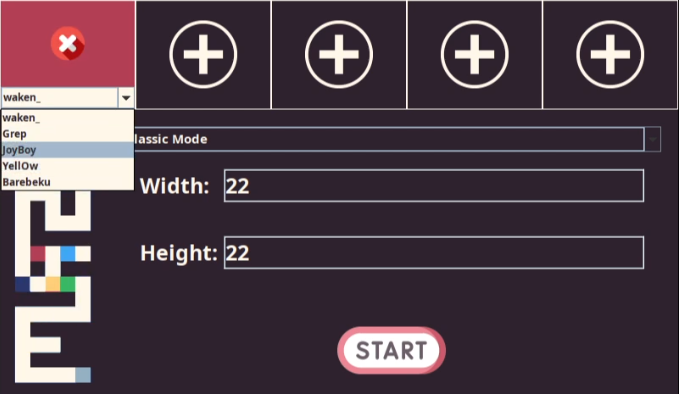
\includegraphics[width=6.5cm]{ressources/Implementation/Labyrinthe/Controleur/SettingsMenu_PlayerList.png}%
        \caption{Liste des joueurs disponibles}
        \label{fig:PlayersAvailable}
    \end{subfigure}
    \qquad
    \begin{subfigure}{6.5cm}
        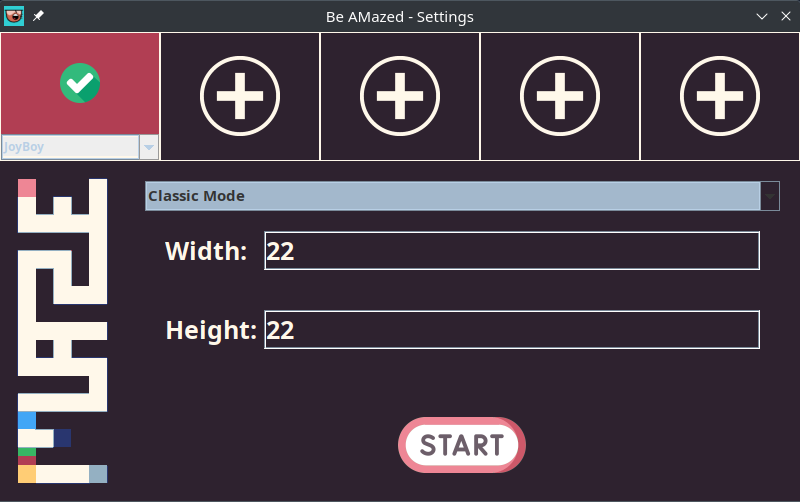
\includegraphics[width=6.5cm]{ressources/Implementation/Labyrinthe/Controleur/SettingsMenu_Ready.png}%
        \caption{Joueur prêt}
        \label{fig:PlayerReady}
    \end{subfigure}
    \caption{Ajout d'un joueur}
    \label{fig:PlayerSelection}
\end{figure}
\FloatBarrier

\paragraph{Lancement de la partie}

Pour lancer la partie on clique sur le bouton
\vcenteredinclude[height=5mm]{ressources/Implementation/Labyrinthe/Controleur/StartButton.png}
après que tous les joueurs soient prêts et que les paramètres précédents aient été choisis.